\documentclass[a4paper, 12pt]{article}
\usepackage{mathptmx}
\usepackage[utf8]{inputenc}
\usepackage[T1]{fontenc}
\usepackage[francais]{babel}
\usepackage{url}
%\usepackage{setspace}

\usepackage{geometry} % see geometry.pdf on how to lay out the page. There's lots.
\geometry{a4paper} % or letter or a5paper or ... etc
% \geometry{landscape} % rotated page geometry

\usepackage{libertine}
\usepackage[pdftex]{graphicx}

\setlength{\parindent}{0cm}
\setlength{\parskip}{1ex plus 0.5ex minus 0.2ex}
%\newcommand{\hsp}{\hspace{20pt}}
\newcommand{\HRule}{\rule{\linewidth}{0.5mm}}



\title{application du UML dans la conception d’une application d’antivol des appareils électroniques : CAS DES SMARTPHONES }

\date{} % delete this line to display the current date

%%% BEGIN DOCUMENT
\begin{document}




\begin{titlepage}
  \begin{sffamily}
  \begin{center}

    % Upper part of the page. The '~' is needed because \\
    % only works if a paragraph has started.
%    \includegraphics[scale=0.04]{logo.png}~\\[1.5cm]

    \textsc{\LARGE Université Libre de Bruxelles}\\[2cm]

    \textsc{\Large Cours: Architecture des Systèmes d'Information}\\[1.5cm]

    % Title
    \HRule \\[0.4cm]
    { \huge \bfseries application du UML dans la conception d’une application d’antivol des appareils électroniques : CAS DES SMARTPHONES }\\[0.4cm]

    \HRule \\[2cm]


    % Author and supervisor
    \begin{minipage}{0.4\textwidth}
      \begin{flushleft} \large
        Etudiant\\
        KETCHADJI KOUTOUDJI ARIANE, 2022-2023\\
      \end{flushleft}
    \end{minipage}
    \begin{minipage}{0.4\textwidth}
      \begin{flushright} \large
        \emph{Professeur :} Monsieur   DE VALERIOLA Sébastien\\
       
      \end{flushright}
    \end{minipage}

    \vfill

    % Bottom of the page
    {\large Année Académique 2022 - 2023}

  \end{center}
  \end{sffamily}
\end{titlepage}





\newpage
\renewcommand{\contentsname}{Sommaire}
\setcounter{tocdepth}{4}
\tableofcontents
\newpage

\section{Introduction}
\quad Les cambriolages effrénés dans les maisons, les boutiques, les magasins et supermarchés, les véhicules… ont poussés les chercheurs à réfléchir sur le moyen d’éradiquer ce problème. C’est ainsi qu’est né le système d'antivol. Ces systèmes ont évolué avec le temps. On est passé des systèmes mécaniques aux systèmes électroniques \footnote{https://www.idisec.com/fr/solutions-antivol-pour-magasins-delectronique }.

\quad Aujourd’hui avec l’avènement des technologies de l’information et de la communication, ces systèmes d’antivols sont appliqués au monde de la téléphonie (Léa Delpont,2019)\footnote{Rakwin, l'antivol connecté pour les téléphones portables | Les Echos } qui, a-t-elle aussi connue une avancée énorme. L’avènement des smartphones va faire de ceux-ci un besoin indispensable pour les hommes et des véritables cibles des personnes mal intentionnées et ce qui va conduire au développement d’applications et systèmes d’exploitation mobiles plus sophistiqués \footnote{http://www.monpetitmobile.com/choisir-mobile/systemes-exploitation-smartphones visité le 12 decembre 2022 à 04h 35 minute
}. \\

\quad Le phénomène de vol de téléphone est un phénomène actuel et courant dans notre Société, chaque jour au moins une personne est victime de vol de téléphone. Les téléphones font partie intégrante de notre vie, ils renferment généralement des données très sensibles. La perte de ces outils emporte donc une partie de nous car elle engendre la perte des données importantes telles que l’annuaire téléphonique, les documents importants, les photos etc. 
Ce qui peut nous faire perdre d’énormes opportunités et un manque à gagner parce qu’on n’a pas pu honorer à un rendez-vous important par exemple. Sans oublier que ces données peuvent aussi être utilisées de manière abusive (vulgarisation ou publication de vos photos ou informations privée) par le détenteur. Comment faire face à ce problème ? De nombreux développeurs d’application, proposent aujourd’hui des applications d’antivol pour smartphones (Jason Champagne, 2015)\footnote{Jason Champagne, Toute l’histoire et la chronologie d’Android, le 24-09-2015} et lorsque nous menons une étude systématique de ces applications, nous constatons que la plupart sont destinés à prendre contrôle de l’appareil à distance c’est-à-dire Verrouiller, bloquer ou effacer son téléphone à distance. En outre, ces services sont cachés et donc pas facile d’accès et requièrent une connexion Internet permanente. 

Par ailleurs lorsque nous sommes victime de vol de notre téléphone ; il est de coutume pour les forces de l’ordre de faire des réquisitions (adressées aux opérateurs de téléphonie) pour avoir le numéro de la nouvelle personne utilisant ce dernier \footnote{Perte ou vol de votre GSM ou de votre smartphone | Bruxelles-Ouest (police.be)} . Il se peut aussi que par moment on ait perdu la facture portant généralement le numéro de série du dit téléphone à retrouver. La réquisition
qui permet d’obtenir le listing ou le contact de celui qui utilise nouvellement le téléphone volé prend généralement trop de temps à faire surface. Il y a donc lieu de s’interroger. Comment peut-on faciliter l’obtention du contact de celui qui utilise nouvellement le téléphone y compris le numéro de série de ce dernier  ? Comment permettre aux forces de l’ordre d’accélérer leur enquête afin de permettre à une victime de rentrer en possession de son appareil ?il sera dont nécessaire de Concevoir et réaliser une application d’antivol  des smartphones pour repondre a toutes ces différentes interrogations.Mais selon les dévéloppeurs d'application, Analyser et concevoir une application fait appel aux méthodes et langages modélisation surtout orientés objet \footnote{NOUMBO NGUETSOP Stephane Cedric MAKA MAKA Ebenezer,Conception et la réalisation d'une application de gestion du presse-papier de windows 7, mémoire  online en informatique et Télécommunications,2013 page 34}.C'est dans cette optique que le thème intitulé de mon article est : Application du UML Dans la Conception d’un Système d’antivol des appareils électroniques : cas des smartphones.

\quad Notre première section sera consacrée à l’état de l’art, nous aborderons l'origine,l'importances et la mise en oeuvre des systèmes d'antivols. La deuxième section de notre étude sera concentrée à l'etat de l'existant sur les applications d'antivols de smartphones nous aborderons l'etude de quelques applications d'antivol de smartphones et les méthodes d'analyses et de conception. La troisième section sera concentrée sur l'analyse et la conception qui consistera a faire une bref présentation de UML,définir les vues répresenter  les diagrammes et le schéma fonctionnel. 



\newpage
\section{Etat de l'art sur les systèmes d'antivol}
Il est question dans ce chapitre de présenter les systèmes
d’antivol tout en dégageant l’importance de ces systèmes.

\subsection{Origine des systèmes d'antivol}

 \quad Au fur et à mesure que le temps passe,le phénomène de vol de téléphone ne fait que s'accentuer dans nos diverses sociètés.c'est ainsi que Les chercheurs, inventeurs et développeurs du 19è siècle vont se mettre ensemble pour trouver des moyens efficaces pouvant palier à ce problème de braquage:d'ou le système d'antivol \footnote{http://blog.labelhabitation.com/decouvrez-lhistoire-de-lalarme-1ere-partie}. Cependant le groupe Abus raconte l'histoire du prémier système d'alarme «\textit{le tout premier brevet du premier système d’alarme électromagnétique du monde fût déposé le 21 juin 1853 par un certain Augustus Russell Pope, inventeur originaire de Somerville dans les environs de Boston . Jusque-là, les gens se fiaient principalement aux cris de leurs voies effrayées, à l’incorruptibilité de leurs chiens de garde ou aux sonnettes mécaniques pour surprendre les cambrioleurs qui s’aventuraient sur leur propriété }»\footnote{https://L’histoire du système d’alarme - Installations d'alarme (abus.com)}.La particularité de la découverte de Pope était que le fait de fermer simplement les porte et les fenetres ne garantir pas que l’alarme devait être arrêtée. .Aujourd’hui un autre est reconnu comme le père du système d’alarme moderne Bien que Pope avait pris en chargé le travail de pionnier\footnote{https://L’histoire du système d’alarme - Installations d'alarme -prototype de pope(abus.com)} .[0.25cm]

 
\quad En effet, Edwin Holmes,richissime entrepreneur et fondateur de la première entreprise de systèmes d’alarme électriques, avait racheté le brevet de Pope en 1857.Et a commencé à exploiter  ceci dans sa société\textbf{«Holmes Electric Protection Company »} \footnote{ https://www.holmeselectricsecurity.com/company-history }.  grâce à sa brillante idée de lier directement son système d'alarme à son lieu de travail,les cables disposés partout dans la ville permettait qu'i recevait directement tous les appels des utilisateurs.c'est ainsi que les habitants de new york ont pu profiter d'un système d'alarme maison liès directement avec la station central (carole, 2017). \\[0.25cm]Après holmes, l’histoire des dispositifs d’alarme modernes fut marquée  par un jeune télégraphiste le nommé d’Edward A. Calahan en 1867.Bien qu'il était sur le point de dévélopper un  projet,qui consistait à rélier 50 maisons entres-elles après qu'il les a équipés d'un boitier d'appel d'urgence et d'une cloche,Mais ayant une autre idée plus sophistiqué,il s'est lancé dans la création d'un système qui permet de déclencher en même temps une alerte et de bénéficier d'un sécour.Pour le réalisé une centrale d'appel était nécessaire car elle réagirait aux appels à l'aide lancé,c'est ainsi qu'il décida de diviser new york en districts,chacun étant relié à une centrale d'appel d'urgence car lorsqu'un appel d'aide est sollicité des garçons de course sont chargés d'aller demandé de l'aide le plus rapide possible pour le district concerné\footnote{Découvrez l'histoire de l'alarme (2e partie)(labelhabitation.com)}. Abus.com explique que « \textit{ L’avantage des boîtiers d’appel d’urgence était qu’ils ne nécessitaient que peu d’entretien. Ils étaient alimentés par le réseau d’alimentation électrique de la gare centrale. Les boîtiers d’appel d’urgence du type Calahan devinrent standards pour la police, les pompiers, et même les services de renseignements} » \footnote{https://L’histoire du système d’alarme - Installations d'alarme -la central d'appel d'urgence(abus.com)} .

\textbf{De nouveaux systèmes d’alarme haute technologie du 20è siècles jusqu'a nos jours}
Dépuis les années1970 jusqu'a nos jours,les systèmes d'alarme n'ont pas cessé de s'améliorer,le premier détecteur de mouvement furent crée en 1970 qui sont intégrés aux systèmes d'alarme et ont révolutionné l'univers de la sécurité en permettant le déclenchement de l'alarme en cas d'intrusion (carole,2017),aussi le système qui se sont démocratisés ont volé la vedette aux système filaire vue son installation beaucoup plus facile et rapide ,de même après les RTC(Réseau Téléphonique Commuté les alertes sont envoyées par réseau téléphonique filaire) ont parle maintenant d'alarmes GSM (permettant d'envoyer les alertes pas mobiles) et enfin les fabricants propose des systèmes d'alarme qui sont de plus en plus performants et intélligents (carole,2017).C’est ainsi que les dévéloppeurs d'abus-security-center il y'a quelque années ont réussi dans un même système d'alarme à intégrer dans la technique d'alarme sans fil moderne une combinaison de protection mécanique et électronique.Abus.com explique l'objectif de ce nouveau système comme « Ceci permet de repousser les tentatives de cambriolage à l’aide d’une résistance mécanique élevée et en même temps de les détecter électroniquement » \footnote{https://L’histoire du système d’alarme - Installations d'alarme -Systèmes d’alarme haute technologie(abus.com}. 
\quad Avec l'évolution technologique ils éxistent plusieurs types d'alarmes de tout types qui sont disponibles sur le marché par exemple l'alarme incendie,alarme piscine etc.Carole justifie cela en disant « Vous l’aurez compris, même si elles ont la même fonction, les alarmes les plus récentes n’ont rien à avoir avec les alarmes des siècles précédents. Si l’on tient compte de l’avancée de la technologie, une chose est certaine : l’alarme maison a encore de belles années devant elle »\footnote{http://blog.labelhabitation.com/systemes-dalarme-lhistoire-depuis-1970-jusqua-nos-jours }.Les chercheurs ne vont pas se limiter aux systèmes d’alarmes ils vont étendre des recherches dans d’autres domaines notamment celui de la téléphonie avec l’ampleur des cas de vol de smartphones pas exemple de l'antivol Rakwin qui a été mis sur pied pas Deux ingénieurs lyonnais, Brahim et Mehdi Hannaizi , qui se présente sous la forme d'un porte-clefs connecté \footnote{https://www.lesechos.fr/pme-regions/innovateurs/rakwin-lantivol-connecte-pour-les-telephones-portables-1004384}.
Très convoités, les Smartphones sont la cible de nombreux mal intentionnés. En France, par exemple le vol du téléphone portable est l'une des atteintes aux biens les plus courantes; Un rapport de l'observatoire national de la délinquance et des réponses pénales
évoque que Les femmes et les jeunes ont été les principales victimes des 678 000 vols de téléphones portable recensés en 2014 selon une enquête\footnote{https://www.ouest-france.fr/societe/faits-divers/vols-de-telephones-portables-les-14-25-ans-sont-les-plus-touches-418976}.

\subsection{Importance des systèmes d’antivol des smartphones}

\quad Devenus de véritables mini-ordinateurs portables, les téléphones mobiles que l’on transporte tous les jours possèdent deux caractéristiques : ils coûtent gros et ils contiennent une bonne partie de notre vie privée ou professionnelle sous forme de données. Ces deux caractéristiques sont d’ailleurs les deux choses auxquelles une victime de vol pense lorsque son précieux appareil vient d’être volé \footnote{\url{https://www.frandroid.com/culture-tech/securite-applications/292577_sommaire}} puisqu’ils regorgent des informations personnelles (des contacts, des souvenirs, notre agenda, des informations très importantes…) et personne n'a envie qu'elles tombent entre de mauvaises mains (sans parler du fait que chacun souhaite Légitimement les récupérer), c’est l’une des raisons pour lesquelles nous devons protéger nos smartphones. Cependant, il est à noter que l’antivol dépend de l’objet qu’on veut protéger et de la Plateforme dans laquelle on se trouve.

\subsection{Mise en œuvre d’un système d’antivol}

\quad Selon Wikipédia ,La mise en œuvre d'un système d’antivol peut prendre plusieurs formes à savoir physique, électronique et passive
\footnote{https ://Antivol — Wikipédia (wikipedia.org)}:
\newline
\textbf{La Forme physique}

La mise en oeuvre physique se fait selon le site wikipédia:
\begin{itemize}
\item En annulant la possibilité de bouger l'objet à protéger(cas d'un antivol relier à une baie ) ;
\item En bloquant automatiquement le mouvement de pièces essentielles de l'objet à protéger (par exemple, un antivol des véhicules, qui empêche les roues avant de tourner) ;
\item en amochant l'objet à protéger de telle manière qu'il soit impraticable ou invendable, si on tente de retirer l'antivol sans les outils adéquats (par exemple, les antivols encreurs de vêtements dans les boutiques de mode)\footnote{\url{https://fr.wikipedia.org/wiki/Antivol#Mise_en_oeuvre_physique}}.
\end{itemize}

\textbf{La Forme électronique}

elle s'obtient:

\begin{itemize}
\item En rendant inactif une fonction logique ou un circuit essentielle au fonctionnement de l'objet à protéger (par exemple, un système anti-démarrage sur une autobus);
\item lorsque l'alarme déclenche ,car il y'a eu tentative de vol sur l'objet protégé ou si la surface délimité pas le détecteur à été franchit par l'antivol en utilisant la technologie radiofréquence exemple : le vol à l'étage;Il existe de très nombreuses variétés d'antennes, qui permettent de rendre le système antivol moins agressif pour la clientèle.\footnote{\url{https://fr.wikipedia.org/wiki/Antivol#Mise_en_oeuvre_électronique}}.Selon un groupe d'ingénieur c'est grace à La technologie radiofréquence identificateur qu'il y 'a échanges entre l'intérrogateur et l'antenne du lecteur ;c'est ainsi qu'il le définisse comme étant « une méthode mise en œuvre pour stocker et récupérer des données à distance en utilisant des marqueurs appelés Transpondeurs ou tags (anglicisme signifiant  étiquette ) et des lecteurs (interrogateurs) » \footnote{SEBAPO Jean-Louis,DAGBA Théophile,ADEDJOUMA A.Sèmiyou,GNACADJA Gilles,SOGBOHOSSOU Médésu:Etude des technologies d’identification par fréquence radio, mémoire de fin de Formation d’Ingénieur de Conception en Réseaux et Télécommunications,2010}.
\end{itemize}

\textbf{La Forme passive}

Elle s'obtient lorsque la remise sur le marché de l'objet volé est plus difficile ou plus couteux; c'est le cas des marquages antivol et des dispositifs d'émission de signaux de localisation, ayant pour but de décourager le vol par les contraintes qui sont posés sur le produit volé \footnote{\url{https://fr.wikipedia.org/wiki/Antivol#Mise_en_oeuvre_passive}}.En effet le marquage permet au propriétaire de l'appareil de rétrouver son appareil, car ce marquage est une preuve pour prouver aisement qu'un bien nous appartient;elle peut etre obligatoire (lorsque après achat d'un objet ou appareil neuve ,elle systématiquement marquées soit pas le fabriquant, soit chez le distributeur )ou facultative  \footnote{Fredéric Heran :LE VOL DE BICYCLETTES : ANALYSE DU PHENOMENE ET METHODES DE PREVENTION , Rapport final ,2003}. 


La suite de notre rédaction nous conduira donc vers une
étude des systèmes d’antivol utilisables sur les smartphones en général.
\newline
\newline
\section{Etat de l'éxistant sur les applications d'antivols de smartphone}

\quad La plupart des applications d’antivol de smartphones propose une fonctionnalité de géolocalisation permettant ainsi de localiser l’objet volé sur une carte en utilisant le réseau GSM ou encore l’option GPS intégré aux smartphones (FREDERIC EVENNOU,2007). Il est donc question pour nous dans cette partie de débuter notre étude par une bref présentation générale de la géolocalisation ; ce qui nous permettra de mieux comprendre la raison de l’implémentation d’une telle fonctionnalité
dans une application d’antivol. Bien après nous ferons une étude de quelques applications d’antivol existant sur le marché.enfin nous faisons une bref présentations des méthodes d'analyses et de conception.
\newline
\subsection{La géolocalisation}
\quad C’est une technologie dont le but est de déterminer la localisation d’un objet ou d’une personne avec une certaine précision,selon le site Techno-Science.net « est un procédé permettant de positionner un objet (une personne, une information, ...) sur un plan ou une carte à l'aide de ses coordonnées géographiques »\footnote{https://www.techno-science.net/glossaire-definition/Geolocalisation.htm}. La technologie insiste fréquemment sur le système GPS (Global Positionning  System) ou sur les interfaces de communication d’un téléphone mobile.  la géolocalisation à des applications multiples tel que:de l’assistance à la navigation, à la mise en relation des personnes, mais aussi à la gestion en temps réel des moyens en personnel et en véhicules des entreprises (OUSSAMA ABDELHAK 2019).Cependant ils existent plusieurs techniques de la géolocalisation dont les plus important sont : la géolocalisation pas satellite,pas GSM,pas WIFI, pas Adresse IP \footnote{OUSSAMA et ABDELHAK :Conception et développement d’une application android pour le suivi des objets mobiles, Mémoire de Fin d’études En vue de l’obtention du diplôme de Master en informatique,2018/2019 Page3}.
\begin{itemize}
\item la géocalisation par satellite
\end{itemize}
\quad Son role est de situer un terminal équipé d'une puce sur la face terrestre(OUSSAMA et ABDELHAK, 2019).Il devra exister une compatibilité avec les signaux émis par une constellation de satellites prévue pour l'occasion avec cette puce.Une position est détectée et est alors traduite en termes de latitude, longitude et parfois altitude et est pret à être représentée physiquement sur une carte;cette technique est utilisée par plusieurs système donc le plus connu est le système américain GPS\footnote{OUSSAMA et ABDELHAK :Conception et développement d’une application android pour le suivi des objets mobiles, Mémoire de Fin d’études En vue de l’obtention du diplôme de Master en informatique,2018/2019 Page4}.
\begin{itemize}
\item la géocalisation par GSM
\end{itemize}
\quad En anglais GSM signifie Global Positionning Recepteur selon le site techno-Science.net,cette technique permet « permet le positionnement d'un terminal GSM en se basant sur certaines informations relatives aux antennes GSM aux quelles le terminal est  connecté » \footnote{https://www.techno-science.net/glossaire-definition/Geolocalisation/gsm.htm}.le GSM est un modèle pour les
communications de téléphonie mobile;ils existent plusieurs technique de localisation tel que des méthodes d’identification de la cellule dans laquelle se trouve le mobile (méthode de Cell ID ou Cell Identification),des méthodes plus complexes basées sur des mesures temporelles (estimation de la distance entre chacune des stations de base et le mobile) comme TOA (Time Of Arrival) ou TDOA (Time difference Of Arrival)et l’utilisation des directions d’arrivée avec la méthode AOA (Angle Of Arrival) conduit aussi à l’identification de la position occupée par le mobile \footnote{FREDERIC EVENNOU. « Techniques et technologies de localisation avancées pour terminaux mobiles dans les environnements indoor » Thèse de doctorat, Grenoble Université Joseph Fourier, 2007, p. 209}.
\begin{itemize}
\item la géocalisation par WIFI
\end{itemize}
\quad La géolocalisation par wifi fonctionne de la Même façon qu'un terminal GSM qui peut se localiser grâce à la méthode du cell ID sur un réseau GSM,un terminal wifi peut adopter la Même methode en s'appuyant sur les identifiants des bornes wifi(adresse MAC)qu'il détecte \footnote{https://www.techno-science.net/glossaire-definition/Geolocalisation/wifi.htm}.
\begin{itemize}
\item la géocalisation par adresse IP
\end{itemize}
\quad C'est une technique qui consiste à s'appuyer sur l'adresse IP pour déterminer la position géographique d'un ordinateur ou de n'importe quel terminal connecté à internet(OUSSAMA et ABDELHAK, 2019). Le principe de cette méthode est de faire une comparaison en temps réel d'un référentiel d'adresse IP comprenant la localisation avec l'adresse IP utilisée par un internaute \footnote{OUSSAMA et ABDELHAK :Conception et développement d’une application android pour le suivi des objets mobiles, Mémoire de Fin d’études En vue de l’obtention du diplôme de Master en informatique,2018/2019 Page5}
\subsection{Étude de quelques applications d'antivol pour smartphones}
\subsubsection{La protection de base d’Android : le gestionnaire d’appareils Android}

\quad Les appareils Android possèdent un Gestionnaire d’appareils Android qui se trouve dans les paramètres Google du téléphone. Ce catalogue réservé permet de configurer son compte Google. Pour le cas de la sécurité antivol, vous pouvez aviver les deux principales options de sécurité liées à Android, à savoir la localisation de l’appareil à distance et l’autorisation de verrouillage et de suppression de l’appareil à distance. Ces deux options permettent de savoir où se trouve son téléphone et de réaliser une réinitialisation de celui-ci à distance\footnote{\url{https://www.frandroid.com/culture-tech/securite-applications/292577_vol-de-smartphone-fonctionne-gestionnaire-dappareils-android-completer}}.Nous énumerons quelques avantages et inconvénients.
\newline
\textbf{Avantages}

On en distingue deux principales à savoir :
\begin{itemize}
\item possibilité de localiser son téléphone ;
\item contrôle du téléphone à distance \footnote{\url{https://www.frandroid.com/culture-tech/securite-applications/292577_vol-de-smartphone-fonctionne-gestionnaire-dappareils-android-completer}}.
\end{itemize}

\textbf{Inconvénients}

Il en existe plusieurs parmi lesquels :
\begin{itemize}
\item Google ne donne pratiquement aucune indication à propos de ses deux paramètres de protection en plus \footnote{\url{https://www.frandroid.com/culture-tech/securite-applications/292577_vol-de-smartphone-fonctionne-gestionnaire-dappareils-android-}};
\item Ces paramètres sont cachés et donc ne sont pas facilement accessibles;
\item Obligation de detenir un compte Google dans le téléphone ;
\item Une fois l’un de ces deux paramètres activés sur un téléphone, ils sont Automatiquement activés sur tous les prochains autres appareils Android qui sont Liés au compte Google qui les a validés ;
\item Ces paramètres visent plus à réduire à néant le téléphone à distance que le retrouver;
\item Pas d’option d’antivol permettant la récupération du téléphone volé La nécessité de toujours avoir une connexion internet car sinon ils ne vous serviront à rien \footnote{Smartphone — Wikipédia (wikipedia.org)}.  
\end{itemize}

\subsubsection{Les Antivirus (Cas d’Avast! Free Mobile Security anti-theft)}
Présentation

\quad Une application de sécurité invisible qui comprend à la fois un antivirus mobile et un contrôle à distance à n'importe quel moment sans déclencher de notifications sur le téléphone.Il offre des options telles que : la protection antivirus, le rapport d’individualisé, le bouclier Web, le filtrage des appels/SMS, un pare-feu, une Icône de notifications personnalisable, une détection des logiciels potentiellement indésirables et des fonctions Anti-Theft. C’est cette dernière qui nous intéresse. Le composant Anti- Theft est pratiquement invisible des voleurs et offre des options de contrôle à distance (via un portail web ou une commande SMS) pour localiser et retrouver le téléphone 'perdu' \footnote{Eman K. Elsayed , Kamal A. ElDahshan , Enas E. El-Sharawy and Naglaa E. Ghannam « Reverse engineering approach for improving the quality of mobile applications » Copyright 2019 Elsayed et al page 9}. Quelques avantages et inconvénients
\newline
Avantages:
\begin{itemize}
\item Contrôle à distance : possibilité de déclencher des fonctionnalités à distance par des commandes SMS à partir du téléphone d'un ami ou en utilisant l’interface web à l’adresse http://my.avast.com  \footnote{\url{https://support.avast.com/fr/article/android-anti-theft-faq-Qu’est-ce que Contrôle en ligne sur my.avast.com?/#pc}};
\item Géorepérage : possibilité du téléphone d’effectuer des actions spécifiques comme: verrouiller, activer la sirène, envoyer la localisation lorsqu'il quitte un périmètre défini (par exemple, si vous allez dans un café et que vous définissez un périmètre
de 500 m, et que quelqu'un vole votre téléphone et l'emporte au-delà de ce périmètre, il active les actions spécifiées)\footnote{\url{https://support.avast.com/fr-be/article/enable-android-anti-theft/#pc}};
\item Identification à distance : le téléphone peut prendre une photo du voleur lorsqu'il tente de déverrouiller l'appareil (peut utiliser l'objectif avant ou arrière, avec reconnaissance des visages).Peut également écouter et enregistrer des sons;
\item Vérification du mot de passe : marque l'appareil comme étant volé si un mot de passe erroné est entré 3 fois dans un écran verrouillé;
\item Envoie d’un SMS depuis votre téléphone vous indiquant le nouveau numéro qui l’utilise avec sa position exacte;
\item Récupération des données à distance : récupérer les journaux d'appels, les messages SMS et d'autres données personnelles de votre téléphone, par exemple avant d'effacer sa mémoire à distance \footnote{https://royalprice.ru/fr/news/skachat-licenzionnyi-antivirus-avast-dlya-android/}.
 \end{itemize}

Inconvénients:
\begin{itemize}
\item Installation du logiciel complexe ;
\item Obligation de disposer d’une connexion internet;
\item Ces paramètres sont invisibles et donc ne sont pas facilement accessibles;
\item Obligation de disposer d’un contrat de licence pour l’installation de l’application;
\item Limitation des numéros d’alerte à 02 numéros\footnote{https://royalprice.ru/fr/news/skachat-licenzionnyi-antivirus-avast-dlya-android}.
\end{itemize}

\subsection{Besoins fonctionnels auxquels devra répondre l'application à développer}
\quad Ils sont directement liés aux tâches que le logiciel devrait pouvoir exécuter. Notre future application doit pouvoir:
\begin{itemize}
\item Permettre la configuration des informations liées au propriétaire du téléphone (le mot de passe ou code de l’application, le numéro de téléphone du propriétaire, le numéro de série de la puce,…) entrés par l’utilisateur ou propriétaire du téléphone ainsi que les numéros de téléphone qui seront utilisés pour retrouver la position du téléphone ;
\item Permettre de consulter les informations de la carte SIM en se connectant;
\item Vérifier les informations de la SIM présente dans le téléphone et les comparer à celles contenues dans sa base de donnée;
\item Envoyer les messages contenant les coordonnées GPS de la position actuel du téléphone ainsi que le nouveau numéro utilisant le téléphone (en cas d’informations différentes de celles contenu dans la base de donnée) aux différents numéros enregistrés;
\end{itemize}

\subsection{Les méthodes d’analyse et de conception}
\quad Pour les ingénieurs informatiques ,Une méthode d’analyse et de conception a pour objectif de « formaliser les étapes préliminaires du développement d’un système afin de rendre son développement plus fidèle aux besoins de l’utilisateur »\footnote{https://fr.wikipedia.org/wiki/Methode d'analyse et de conception}. Il existe plusieurs méthodes d’analyse et de conception à savoir : RACINES, MERISE, NIAM, OMT (Objet Modeling Technique), Booch, UML etc...Chacune de ces méthodes a été mise sur pied pour résoudre un problème persistant(robustesse, maintenance, sécurité…) dans l’industrie du développement du logiciel \footnote{https:// Méthodes d'analyse et de conception : définition et explications (techno-science.net)}. À chaque méthode correspond un ou plusieurs moyens (plus ou moins précis) de représentation des résultats. Celui-ci peut être graphique (diagramme synoptique,organigramme) ou textuel (expression d’un besoin en langage naturel, jusqu’au listing du code source). Le choix de la méthode d’analyse dépend exclusivement des connaissances préalables des membres du groupe ,de meme choisir une méthode qui implique un nouvel apprentissage de celui-ci n’est pas conseillé \footnote{NOUMBO NGUETSOP Stephane Cedric MAKA MAKA Ebenezer,Conception et la réalisation d'une application de gestion du presse-papier de windows 7, mémoire  online en informatique et Télécommunications,2013 page 32}. En fonction du domaine industriel dans lequel nous voulons travaillé ,des résultats que nous aimerons obtenir et des connaissances dans une methode d'analyse précis , nous avons opté pour la méthode d’analyse UML.


\section{Analyse et Conception}
\quad L’analyse et la conception d’une solution informatique a toujours fait preuve de minutie. Elle demande des connaissances particulières sur des méthodes d’analyse,les langages de modélisation \footnote{NOUMBO NGUETSOP Stephane Cedric MAKA MAKA Ebenezer,Conception et la réalisation d'une application de gestion du presse-papier de windows 7, mémoire  online en informatique et Télécommunications,2013 page 34}. Il s’agira pour nous dans cette section de faire un bref aperçu de l'outil d'analyse qui doit être utlisé pour implémenter les modules principaux de l'application. Ensuite produire un organigramme de fonctionnement de l'application et enfin présenter ses différentes interfaces.


\subsection{Présentation UML}
\quad UML est un langage graphique de modélisation et est issue en 1997 de la combinaison de trois langages de modélisation (les plus utilisés à l’époque) à savoir : OMT (Object Modeling Technique) de James RUMBAUGH, BOOCH de Grady BOOCH et OOSE (Object Oriented Software Engineering) d’Ivar JACOBSON (Laurent AUDIBERT ,2007). UML, manager par l’OMG (Object Management Group est aujourd’hui le standard de modélisation orienté objet le plus utilisé en génie logiciel et sa version UML-2.1 est la plus répandue et la plus utilisée à nos jours\footnote{NOUMBO NGUETSOP Stephane Cedric MAKA MAKA Ebenezer,Conception et la réalisation d'une application de gestion du presse-papier de windows 7, mémoire  online en informatique et Télécommunications,2013 page 36}. C’est cette dernière que nous utiliserons pour la modélisation de l’application qui ne sera pas implémenté.


\subsection{Les vues et diagrammes d’UML}

\quad UML est un langage graphique, il est donc basé sur l’utilisation des diagrammes; la version UML 2.0 augmente le nombre de diagrammes, qui passe de 9 à 13;Ces diagrammes sont organisés en vues(étant un moyen de décrire un système suivant un angle donné, a chaque vue correspond des diagrammes) UML\footnote{NOUMBO NGUETSOP Stephane Cedric ,MAKA MAKA Ebenezer :Conception et la réalisation d'une application de gestion du presse-papier de windows 7, mémoire  online en informatique et Télécommunications,2013 page 36 (3.1.2. Les vues et diagrammes d'UML)}.
UML modélise un système selon trois axes ou vues à savoir : la Vue fonctionnelle ; la vue dynamique  et la vue statique \footnote{ Qu'est-ce que le langage UML ; Lucidchart}.

\subsubsection{La vue fonctionnelle}
\quad Encore appelée vue interactive, elle illustre les interactions entre les différents acteurs/utilisateurs et le système, sous forme d’objectif à atteindre d’un côté et sous forme chronologique de scénario d’interactions typiques de l’autre (Olivier Sigaud,2004). Elle se compose de trois diagrammes : le diagramme des cas d’utilisation, le diagramme des séquences, diagramme de classe\footnote{Olivier Sigaud : Introduction à la modélisation orientée objets avec UML, support de cours « Génie Logiciel et Programmation Orientée Objet » de l’ENSTA, 2004}. Pour notre cas nous utiliserons le diagramme des cas d’utilisation.
\newline
\begin{itemize}
\item Diagramme des cas d’utilisation
\end{itemize}
Ces diagrammes à pour but de représenter les exigences du point de vue purement Fonctionnel du système à réaliser. Un cas d’utilisation fait référence à un usage particulier du système utilisé à une fin précise (MAKA,Noumbo,2013).un cas d’utilisation d'après olivier Sigaud « Modélise une interaction entre le système informatique à dévélopper et un utilisateur ou acteur interagissant avec le système » \footnote{Olivier Sigaud : Introduction à la modélisation orientée objets avec UML, support de cours « Génie Logiciel et Programmation Orientée Objet » de l’ENSTA, 2004 page 8}.  Les cas d’utilisation ont plusieurs chemin qui peuvent être représentés sous forme de récits( descriptions de cas d’utilisation ) ou de modèles visuels ( diagrammes de cas d’utilisation ),le choix dépend de l'objectif spécifique à atteindre, et le chemin normale selon cybermediane est « un ensemble d’étapes inconditionnelles qui décrivent comment atteindre les objectifs du cas d’utilisation et satisfaire les intérêts de tous les acteurs principaux ou de soutien concernés. Chaque étape est essentielle pour atteindre les objectifs du cas d’utilisation et aucune des étapes ne peut être ignorée »\footnote{Qu'est-ce qu'un cas d'utilisation dans la modélisation de cas d'utilisation UML ? - Cybermédiane (cybermedian.com)}.

Présentation des cas d’utilisation de l’application
Pour mieux comprendre les cas d’utilisation que nous allons présenter ci-dessous il est intéressant d’identifier chaque acteur avec ses différents rôles pour enfin ressortir facilement ces cas d’utilisation. Pour cela nous avons le tableau ci-dessous:


\begin{tabular}{|p{3.5cm}|p{3.5cm}|p{3.5cm}|}
\hline
\centering ACTEURS & \centering ROLES & \centering CAS D'UTILISATION 
\tabularnewline
\hline
\raggedright Propriétaire & Valider le formulaire d’enregistrement & \raggedright Enregistrer les informations de récupérations 
\tabularnewline
\hline
\raggedright Utilisateur & Valider le formulaire de connexion & Consulter les informations \tabularnewline 
\hline
\centering Système exploitation &\centering Lancer l’application & \begin{itemize} \item Vérifier des informations de la Sim et ceux de la base de données\end{itemize} \begin{itemize}
\item Envoyer le message au cas où les informations vérifiées ne concordent pas 
\end{itemize} \tabularnewline
\hline
\end{tabular}

De ce qui précède il vient que nous avons trois cas d’utilisations nous permettant de déduire le diagramme ci-après
\begin{figure}[h]
\begin{center}
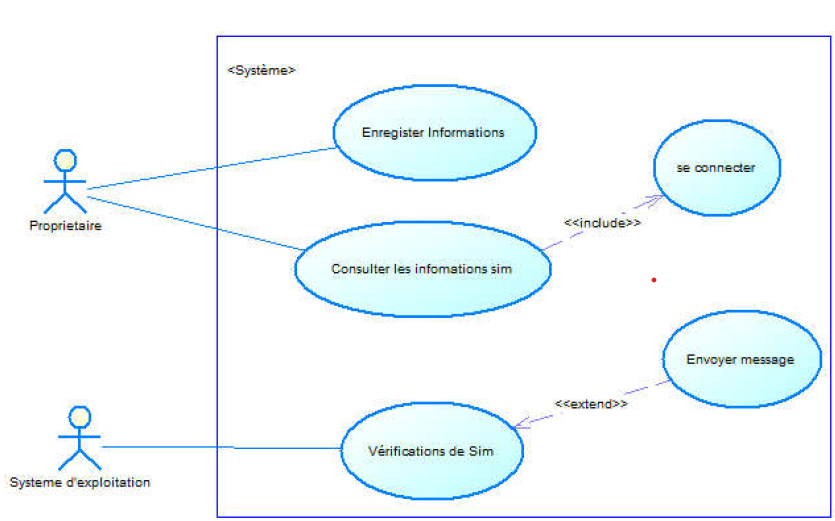
\includegraphics[scale=0.5]{images4.png}
\end{center}
\caption{diagramme des cas d’utilisation.}
\end{figure}


Tous les cas d’utilisation étant recensés et modélisés il est important de décrire les agissements de ces cas d’utilisation d’où la nécessité de la vue dynamique.

\subsubsection{La vue dynamique}
\quad La vue dynamique vise à montrer l’évolution des objets complexes du programme tout au long de leur cycle de vie et est orientée algorithme et traitement ( Noumbo et Maka,2013). De leur naissance à leur mort, les objets voient leurs états changés et ce à cause de leur interaction avec d’autres objets du programme \footnote{NOUMBO NGUETSOP Stephane Cedric ,MAKA MAKA Ebenezer :Conception et la réalisation d'une application de gestion du presse-papier de windows 7, mémoire  online en informatique et Télécommunications,2013 page 39 ( La vue dynamique)}. La vue dynamique est constituée des diagrammes d’états,des diagrammes d’activité, des diagrammes de séquence et des diagrammes de communication\footnote{ Laurent AUDIBERT, UML 2, Édition 2007-2008}. Pour le  cas soumis à notre étude le diagramme de séquence qui convient à nos attentes. \\ 



\begin{itemize}
\item Diagramme de sequence
\end{itemize}

\quad Un diagramme de séquence permet selon AMARA Nesrine:«\textit{de montrer les interactions d'objets dans le cadre d'un scénario d'un diagramme des cas d'utilisation. Dans un souci de simplification, on représente l'acteur principal à gauche du diagramme, et les acteurs secondaires éventuels à droite du système. Le but étant de décrire comment se déroulent les actions entre les acteurs ou objets } »\footnote{AMARA Nesrine:La réalisation d’une application mobile Android communiquant avec un Beacon, Mémoire de Fin d’études En vue de l’obtention du diplôme de Master en informatique,2018/2019 Page36} . De manière chronologique Les diagrammes de séquences mettent en valeur les échanges de messages (déclenchant des événements) entre acteurs et objets (ou entre objets et objets)(Laurent AUDIBERT ,2007/2008).De ce fait comme le souligne oussama et abdelhak :« Chaque cas d’utilisation est décrit textuellement de façon détaillée, mais donne également lieu à un diagramme de séquence simple représentant graphiquement la chronologie des interactions entre les acteurs et le système vu comme une boîte noire, dans le cadre du scénario nominal ».\footnote{OUSSAMA et ABDELHAK :Conception et développement d’une application android pour le suivi des objets mobiles, Mémoire de Fin d’études En vue de l’obtention du diplôme de Master en informatique,2018/2019 Page24}. Les différents diagrammes de séquence de notre application sont présentés sur les figures ci-dessous:

\quad{le diagramme de séquence} lié à l’enregistrement des informations du propriétaire du smartphone au sein de la base de données lors de sa première connexion à l’application (figure 2).\\


\begin{figure}[h]
\begin{center}
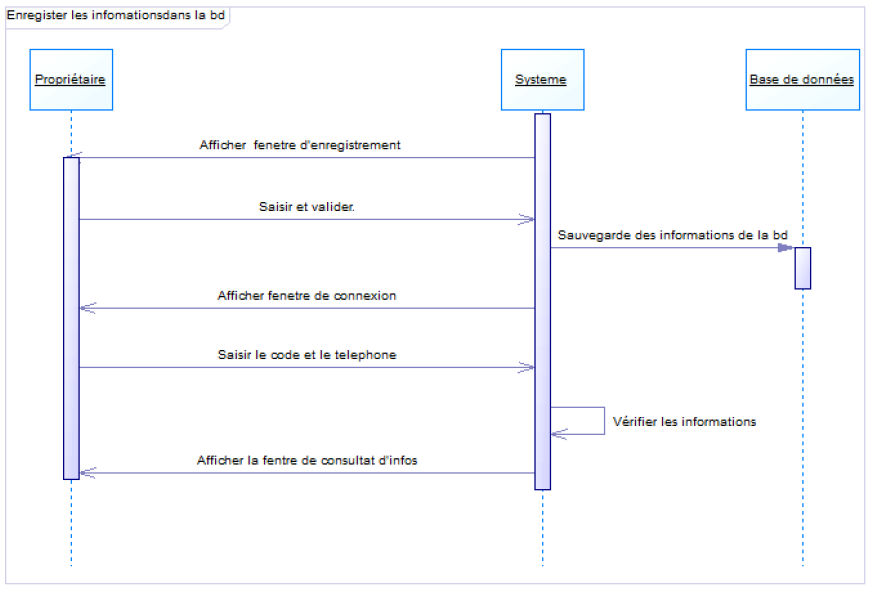
\includegraphics[scale=0.5]{images7.png}
\end{center}
\caption{diagramme de séquence d’enregistrement des informations dans la base de données.}
\end{figure}

\quad {le diagramme de séquence} lié à la consultation des informations du propriétaire du smartphone au sein de la base de données en vue d’une
modification de ces dernières. On suppose que le propriétaire ait envie de modifier un numéro entré lors de la première configuration (figure 3).\\




\begin{figure}[h]
\begin{center}
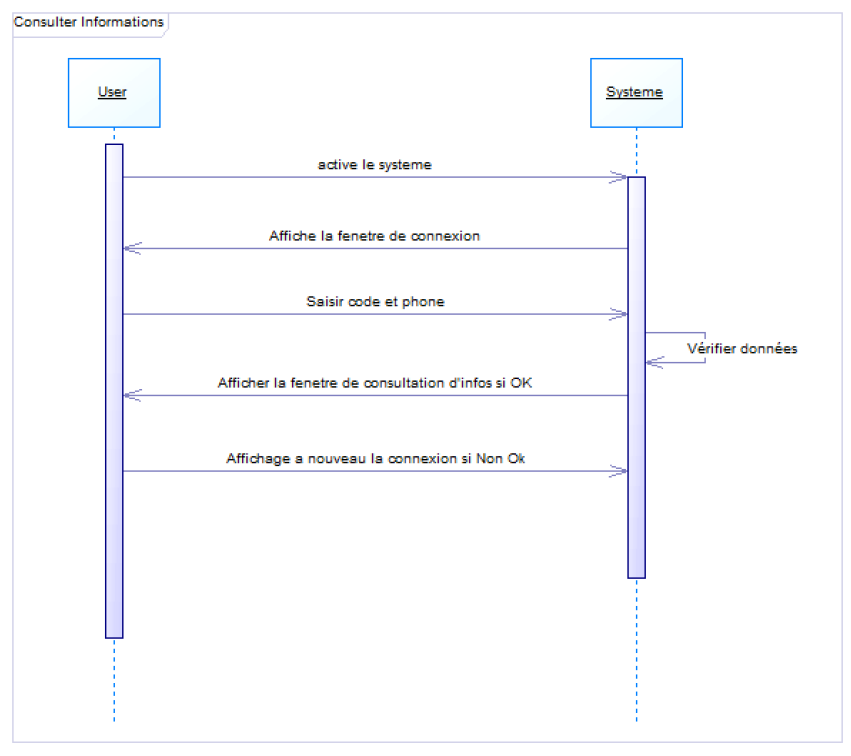
\includegraphics[scale=0.5]{images5.png}
\end{center}
\caption{diagramme de séquence de consultation des informations.}
\end{figure}

\quad {le diagramme de séquence} renfermant la fonctionnalité la plus importante de notre application. Elle présente le diagramme de séquence
lié à la vérification de la carte SIM lors d’un démarrage de l’appareil afin d’envoyer ou non un message d’alerte de changement de SIM aux numéros définis par le propriétaire du téléphone lors de sa première configuration (figure 4).\\



\begin{figure}[htp]
\begin{center}
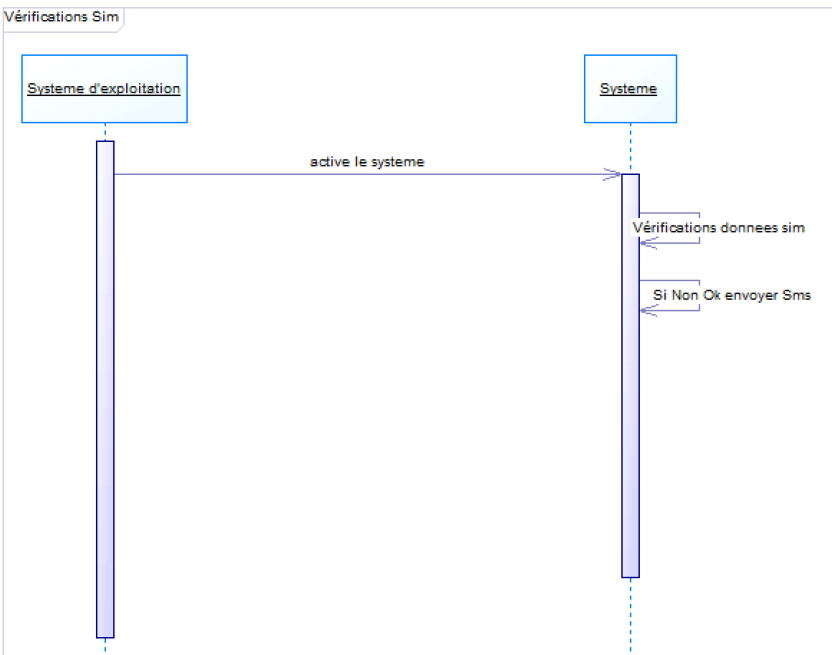
\includegraphics[scale=0.5]{image1.png}
\end{center}
\caption{diagramme de séquence de vérification de SIM et envoie de message d’alerte.}
\end{figure}


Ces diagrammes de séquences nous ont permis d’avoir un comportement détaillé de chaque objet de notre application et de ressortir les différentes méthodes associées à chacun d’eux. Tout ceci étant fait on peut donc présenter la vue statique de notre application.

\subsubsection{La vue structurelle ou statique}
\quad La vue structurelle présente la structuration des données et identifie les objets/composants constituant le programme, leurs attributs, opérations et méthodes, ainsi que les liens ou associations qui les unissent (Pascal Roques,2014).Pour spécifier une application La vue structurelle du modèle UML est la vue la plus utilisée  et elle à pour objectif de modéliser la structure des différentes classes d’une application orientée objet ainsi que leurs relations Elle regroupe également les classes fortement liées entre elles en des composants les plus autonomes possibles \footnote{Xavier Blanc, Isabelle Mounier avec la contribution de Cédric Besse : UML2 pour les développeurs,}. La vue statique est constituée des diagrammes de classes, des diagrammes de packages, des diagrammes d’objets, des diagrammes de structure composite, des diagrammes de déploiement 20\footnote{Qu'est-ce que le langage UML | Lucidchart}.

\begin{itemize}
\item Diagramme de classe
\end{itemize}

\quad Le diagramme de classe décrit le type des objets ou données du système ainsi que les différents formes de rélations statique qui les relient entre-eux (olivier sigaud,2004).De ce fait, d'après Noumbo et Maka «\textit{ est le diagramme le plus important dans la modélisation UML (il est le diagramme prioritaire pour les outils de génération automatique de code). Ces diagrammes sont représentés avec plus ou moins d’exhaustivité selon que l’on est en phase d’analyse, de conception ou d’implémentation} »\footnote{NOUMBO NGUETSOP Stephane Cedric ,MAKA MAKA Ebenezer :Conception et la réalisation d'une application de gestion du presse-papier de windows 7, mémoire  online en informatique et Télécommunications,2013 page 43}. Avant de dessiner un diagramme de classe il est nécéssaire de prendre en compte la phase dans laquelle on se trouve ;alors en phase d’implémentation on cherche à décrire chaque classe, ses attributs et ses méthodes en pensant déjà au code qui les implémentera tout en tenant compte les contraintes matérielles de temps d’exécution, d’architecture, etc \footnote{Pascal Roques : UML par la pratique, 5e Edition, EYROLLES ISBN 2-212-12014-1,2010}.
Voici quelque concepts élémentaires les plus employés 
pour la réalisation de la vue structurelle d’un modèle UML.

\textbf{Classe}
Sémantique

En UML, une classe  permet l'élaboration d’objets instances de cette classe et spécifie la structure commune d’un ensemble d’objets . Une classe est identifiée par son nom (Xavier blanc et isabelle mounier).

Graphique 
Une classe se représente à l’aide d’un rectangle, qui contient le nom de la classe sous forme de tableau à une colonne et trois lignes ; qui contient le nom de la classe (première ligne et
éventuellement le nom du package auquel elle appartient) viennent ensuite les propriétés(deuxième ligne) de la classe puis ses opérations (troisième ligne)\footnote{Xavier Blanc, Isabelle Mounier avec la contribution de Cédric Besse : UML2 pour les développeurs,2010 page 13}. La Figure ci-dessous illustre la classe nommée User

\textbf{Les propriétés ou attributs}
Pour une classe, une propriété peut être aperçu comme une forme élémentaire d’agencement entre les objets (instances) de la classe et un objet de classe standard et les propriétés de la classe sont notées de la façon suivante :

<NomAttribut> : <Type> = [<valeur par défaut>]\footnote{Olivier Sigaud : Introduction à la modélisation orientée objets avec UML, support de cours « Génie Logiciel et Programmation Orientée Objet » de l’ENSTA, 2004 page 13}.
\textbf{Les opérations} 

Une opération peut être aperçu comme un travail que doit exécuter  l’objet lorsqu’on lui fait appel et elle désigne une méthode de la classe En programmation ( Noumbo et Maka,2013). pascal roques décrit comment se fait la notation des opérations et définit les 2 catégories d'opérations « Dans un diagramme de classe  se fait de la façon suivante :

<NomOpération> (ListeParamètres) : <TypeRetour>
On distingue deux catégories d’opérations :

Celles qui changent l’état de l’objet (ses attributs) : ces opérations sont appelées modifiants ou mutateurs.

 À l’opposé des opérations d’accès ou accesseurs qui ne se
contentent que de retourner la valeur d’une propriété »\footnote{Pascal Roques : UML par la pratique, 5e Edition, EYROLLES ISBN 2-212-12014-1}.

De ce qui précède, on a donc la Figure suivante(figure 5)

\begin{figure}[h]
\begin{center}
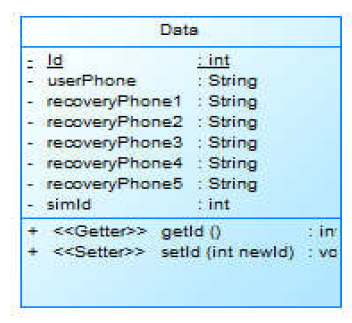
\includegraphics[scale=0.75]{images3.png}
\end{center}
\caption{diagramme de classe de l’application.}
\end{figure}

\subsection{schéma fonctionnel de l'application}



La figure ci-dessous représente le schéma fonctionnel de l’application. Son observation permet de comprendre les différents processus mis en oeuvre pendant le fonctionnement de l’application du redémarrage du téléphone jusqu’à l’envoie du message d’alerte(figure 6)\\





\\
\begin{figure}[h]
\begin{center}
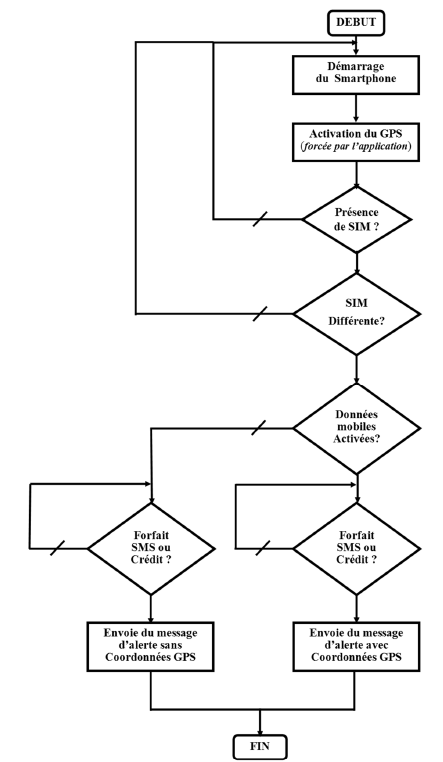
\includegraphics[scale=0.75]{images2.png}
\end{center}
\caption{schéma fonctionnel de l’application.}
\end{figure}\\




\newpage
\section{Conclusion}

\quad Cet article rédigé dans le cadre des travaux patiques du cour d’architecture des systèmes d’information à l’universiré Libre de Bruxelle en vue de l’obtention du Ma-STIC, nous a donné l’occasion de concilier la théorie et la pratique et d’appliquer les connaissances acquises lors des séances de cour.Comme nous l’avons si bien mentionné tout au long de notre travail, les problèmes que pose la perte de Smartphone constituent un point sensible dans la mesure où ces téléphones Renferment généralement nos vies. La perte de ces informations peut nous faire perdre des opportunités énormes et même des informations très capitales. En effet, l’objectif principal de Notre travail portait sur l’application du UML dans la conception d’une application d’antivol des appareils électroniques : CAS DES SMARTPHONES.Plus précisément,UML qui est un langage graphique basé sur l’utilisation des diagrammes( cas d'utilisation,séquences et de classe)nous a permis de concevoir l'application qui permettra de retrouver un téléphone volé grâce à un message envoyé par celui-ci renfermant le numéro du nouvel utilisateur, le numéro IMEI du téléphone et sa position à l’instant t.\\


\quad Ce travail que nous avons effectué de manière méthodique pour atteindre nos objectifs, s’est réalisé par l’intermédiaire de certains outils indispensables. Comme démarche, nous avons d’abord présenté les généralités (origine,importance et mise en oeuvre sur les systèmes d’antivol);l’étude de l’existant qui nous a permis de décrypter certains problèmes que posent  les applications d’antivol pour smartphones , et d’élaborer les besoins fonctionnel de l'application . Nous avons enfin procédé à l'analyse et la conception de notre application par la méthode d’analyse UML .\\

\quad Nous aurions souhaité la réaliser sous Android studio à l’aide des langages JAVA et XML puis étendre cette application dans d’autres plates-formes, faire plus côté sécuritaire en la protégeant d’une désinstallation potentielle et de la suppression voir même une intégration de la gestion du téléphone à distance. Compte tenu du temps que nous n’avons pas assez eu, nous les renvoyons pour des recherches futures.


\newpage
\begin{thebibliography}{9}


\bibitem{refences}
IDISEC.COM: \textit{Solution antivol pour magasins électroniques }[en ligne; consulté le 12-Décembre-2022] \url{https://www.idisec.com/fr/solutions-antivol-pour-magasins-delectronique}
\bibitem{refence1}
Léa Delpont,2019 .Rakwin,l'antivol connecté pour les téléphones portables,28 Mars 2019 .[en ligne; consulté le 12-Décembre-2022]. \url{https://www.lesechos.fr/pme-regions/innovateurs/rakwin-lantivol-connecte-pour-les-telephones-portables-1004384}
\bibitem{refence2}	
MonPetitMobile.com:\textit{Conseil pour choisir les systèmesd'exploitation des smartphone }.copyright 2022[enligne; consulté le 12-Décembre-2022].
 \url{https://www.monpetitmobile.com/choisir-mobile/systemes-exploitation-smartphones}
\bibitem{refence3}
Jason Champagne, 2015. Toute l’histoire et la chronologie d’Android. le 24-09-2015 
\bibitem{refence4}
police.be:\textit{Perte ou vol de votre GSM ou de votre smartphone} [en ligne; consulté le 12-Décembre-2022]. 
\url{https://www.police.be/5340/fr/questions/perte-ou-vol/perte-ou-vol-de-votre-gsm-ou-de-votre-smartphone}
\bibitem{refence4}
NOUMBO NGUETSOP Stephane, Cedric MAKA MAKA Ebenezer. « \textit{Conception et la réalisation d'une application de gestion du presse-papier de windows 7 }» . mémoire  online en informatique et Télécommunications,2013 page (32-35)
\bibitem{refence5}
CAROLE,2017.LABEL HABITATION.\textit{Découvrez l'histoire de l'alarme 1e partie },14Janvier 2017. [en ligne; consulté le 12-Décembre-2022].

\url{http://blog.labelhabitation.com/decouvrez-lhistoire-de-lalarme-1ere-partie/}
\bibitem{refence6}
CAROLE,2017.LABEL HABITATION.\textit{Découvrez l'histoire de l'alarme 1e partie}. 14 Janvier 2017.[en ligne;consulté le 12-Décembre-2022].

\url{http://blog.labelhabitation.com/decouvrez-lhistoire-de-lalarme-2ere-partie/}
\bibitem{refence7}
CAROLE,2017.LABEL HABITATION.\textit{Découvrez l'histoire de l'alarme 1e partie}.14 Janvier 2017.[en ligne;consulté le 12-Décembre-2022].

\bibitem{refence7}
Ouest-france .\textit{Vols de smartphones. Les 14-25 ans et les femmes sont les plus touchés}. 27 Avril 2016. [en ligne; consulté le 13-Décembre-2022].
\url{https://www.ouest-france.fr/societe/faits-divers/vols-de-telephones-portables-les-14-25-ans-sont-les-plus-touches}
\bibitem{refence7}
Holmes security systèmes.\textit{Historique de l'entreprise}.[en ligne; consulté le 15-Décembre-2022].

\url{https://www.holmeselectricsecurity.com/company-history}
\bibitem{refence8}
Techno-Science.net.\textit{Géolocalisation - Définition et Explications}.[en ligne; consulté le 15-Décembre-2022].

\url{https://www.techno-science.net/glossaire-definition/Geolocalisation.html}
\bibitem{refence9}
FRANDROID .COM .\textit{Vol de smartphones : comment fonctionne le gestionnaire d’appareils Android et comment le compléter},4 Juillet 2015.[en ligne; consulté le 15-Décembre-2022].
\url{https://www.frandroid.com/culture-tech/securite-applications/292577_vol-de-smartphone-fonctionne-gestionnaire-dappareils-android-completer}
\bibitem{refence10}
WIKIPEDIA encyclopedie libre.\textit{Antivol}.[en ligne; consulté le 15-Décembre-2022].
\url{https://fr.wikipedia.org/wiki/Antivol}
\bibitem{refence11}
SEBAPO Jean-Louis,DAGBA Théophile,ADEDJOUMA A.Sèmiyou,GNACADJA Gilles et SOGBOHOSSOU Médésu. « \textit{Etude des technologies d’identification par fréquence radio}». Mémoire de fin de Formation d’Ingénieur de Conception en Réseaux et Télécommunications et Télécommunications,2013 page 34
\bibitem{refence11}
Fredéric Heran . « \textit{LE VOL DE BICYCLETTES : ANALYSE DU PHENOMENE ET METHODES DE PREVENTION}» .Rapport final fevrier 2013
\bibitem{refence12}
Hamimes OUSSAMA et Kedadra ABDELHAK. « \textit{ Conception et développement d’une application android pour le suivi des objets mobiles} » . Mémoire de Fin d’études En vue de l’obtention du diplôme de Master en informatique . 2018/2019
\bibitem{refence13}
Eman K. Elsayed , Kamal A. ElDahshan , Enas E. El-Sharawy and Naglaa E. Ghannam .\textit{ Reverse engineering approach for improving the quality of mobile applications }.Copyright 2019 Elsayed et al page 9 
\bibitem{refence14}
AVAST.\textit{Avast Mobile Security pour Android}.1988-2022 Copyright Avast Software SRO.[en ligne; consulté le 18-Décembre-2022]
\url{https://support.avast.com/fr-be/article/android-anti-theft-faq/#pc}
\bibitem{refence14}
AVAST.\textit{Activation de l'Antivol dans Avast Mobile Security}.1988-2022 Copyright Avast Software SRO .[en ligne; consulté le 18-Décembre-2022]

\url{https://support.avast.com/fr-fr/article/enable-android-anti-theft/#pc}
\bibitem{refence13}
ROYALPRICE.\textit{Télécharger l'antivirus sous licence avast pour android}.[en ligne; consulté le 18-Décembre-2022]

\url{https://royalprice.ru/fr/news/skachat-licenzionnyi-

antivirus-avast-dlya-android/}
\bibitem{refence10}
WIKIPEDIA encyclopedie libre.\textit{Methode d'analyse et de conception}.[en ligne; consulté le 16-Décembre-2022]

\bibitem{refence13}
Eman K. Elsayed , Kamal A. ElDahshan , Enas E. El-Sharawy and Naglaa E. Ghannam .\textit{ Reverse engineering approach for improving the quality of mobile applications }.Copyright 2019 Elsayed et al page 9 
\bibitem{refence14}
AVAST.\textit{Avast Mobile Security pour Android}.1988-2022 Copyright Avast Software SRO.[en ligne; consulté le 18-Décembre-2022]
\url{https://support.avast.com/fr-be/article/android-anti-theft-faq/#pc}
\bibitem{refence14}
AVAST.\textit{Activation de l'Antivol dans Avast Mobile Security}.1988-2022 Copyright Avast Software SRO .[en ligne; consulté le 18-Décembre-2022]

\url{https://support.avast.com/fr-fr/article/enable-android-anti-theft/#pc}
\bibitem{refence13}
ROYALPRICE.\textit{Télécharger l'antivirus sous licence avast pour android}.[en ligne; consulté le 18-Décembre-2022]

\url{https://royalprice.ru/fr/news/skachat-licenzionnyi-

antivirus-avast-dlya-android/}
\bibitem{refence10}
WIKIPEDIA encyclopedie libre.\textit{Methode d'analyse et de conception}.[en ligne; consulté le 16-Décembre-2022]
\url{https://fr.wikipedia.org/wiki/Methode d'analyse et de conception}.
\bibitem{refence14}
Techno-Science.net.\textit{Méthodes d'analyse et de conception : définition et explications}.[en ligne; consulté le 18-Décembre-2022]
\url{https://www.techno-science.net/definition/749.html}
\bibitem{refence15}
Lucidchart.\textit{Qu'est-ce que le langage UML}.[en ligne; consulté le 18-Décembre-2022]
\url{https://www.lucidchart.com/pages/fr/langage-uml}.
\bibitem{refence15}
Cybermédiane.\textit{Qu'est-ce qu'un cas d'utilisation dans la modélisation de cas d'utilisation UML}.07 Mars 2022 [en ligne; consulté le 20-Décembre-2022]

use-case-modeling/}
\bibitem{refence16}
Olivier Sigaud .\textit{Introduction à la modélisation orientée objets avec UML}.support de cours « Génie Logiciel et Programmation Orientée Objet » de l’ENSTA, 2004.
\bibitem{refence16}
Laurent AUDIBERT.\textit{UML 2 de l'apprentissage à la pratique}.Édition 2007-2008
\bibitem{refence17}
AMARA Nesrine.«\textit{La réalisation d’une application mobile Android communiquant avec un Beacon} ».Mémoire de Fin d’études En vue de l’obtention du diplôme de Master en informatique . 2018/2019
\bibitem{refence18}
XAVIER BLANC,Isabelle Mounier avec la contribution de Cédric Besse.\textit{ UML 2, pour les développeurs}.Paris : Éditions Eyrolles, 2006.
\bibitem{refence18}
Pascal Roques.«\textit{UML par la pratique}. paris: 5e Edition, EYROLLES ISBN 2-212-12014-1,2010


\end{document}
